% !TEX root = QlockToo.tex
\begin{multicols}{2}
\section{Elektronik}
\label{sec:Elektronik}
Während Konstruktion und die Basisfunktionen der Worduhr sich sehr eng am Original orientieren, ist die Umsetzung in der Elektronik komplett selbst entwickelt.

\textbf{LED-Matrix}

Die LED-Matrix mit 10~x~11 Pixel wird von einem Mikrocontroller angesteuert. Dies geschieht zeilenweise im Multiplexing-Verfahren. Hierbei wird die erste Zeile von einem Transistor mit Spannung versorgt. Die 11 Pixel der Zeile werden über einen LED-Treiber simultan angesteuert. Nach einer Millisekunde wird die Zeile ausgeschaltet, es werden neue Daten in den LED-Treiber geschrieben und die nächste Zeile wird eingeschaltet. 

\textbf{Arduino Mirco}

Als Mikrocontroller wird ein Arduino Micro Board mit dem Atmel Atmega 32U4 Controller verwendet. Der Einsatz eines Arduino Boards vereinfacht die Umsetzung einer seriellen Schnittstelle und verringert durch das bereits vielfach genutzte Board die Fehlerquellen im Layout. Durch die kleine Bauform und die sich aus den Features ergebenden Anforderungen (serielle Kommunikation, $I^{2}C$-Bus, externer Interrupt, 4x Digital Input 2x Analogeingang und 10x Digital Output) fiel die Auswahl auf den Arduino Micro.

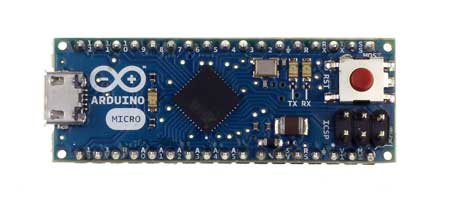
\includegraphics[width=\columnwidth]{Abbildungen/Elektronik/ArduinoMicro}

\textbf{LED-Treiber}

Der TLC59116 LED-Treiber von Texas Instruments hat 16 PWM-Ausgänge mit 8Bit Auflösung - 255 Helligkeitsstufen - und eine Stromregelung, die es ermöglicht auf Vorwiderstände an den LED zu verzichten. Der IC wird über $I^{2}C$ angesteuert.Die Adresse kann hardwareseitig in den letzten 4Bit eingestellt werden und ist auf der Platine hart mit 0b1100 000[R/W] adressiert. Der LED-Treiber ist in der SMD TSSOP-28 Bauform.

\textbf{Transistoren}

Die Zeilen werden mit IRF7416 P-FET-Transistoren geschaltet und mit $5V$ versorgt. Die Transistoren werden mit einem Pull-Up Widerstand am Gate beschaltet und mit einem invertierten Signal angesteuert (4~-~13). Die Transistoren haben S0-8 Gehäusebauform. 

\textbf{Taster}

{
\centering 
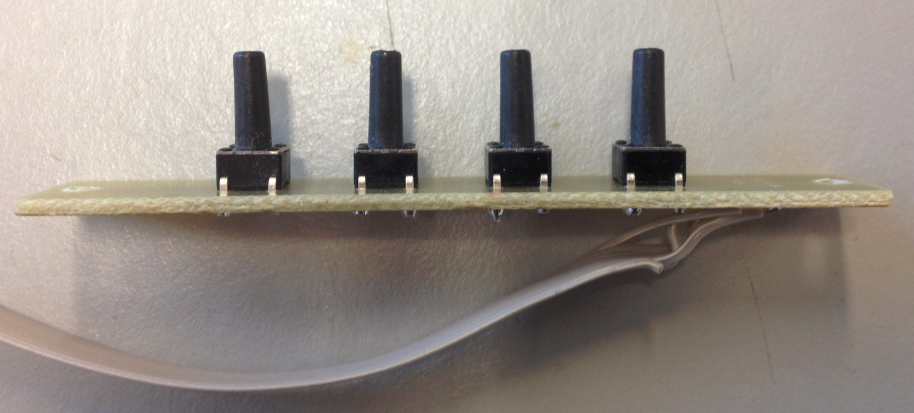
\includegraphics[width=0.9\columnwidth]{Abbildungen/Konstruktion/Taster02} 
}

{
\centering 
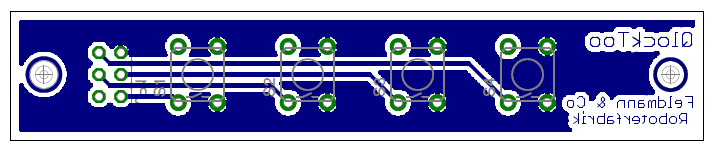
\includegraphics[width=0.9\columnwidth]{Abbildungen/Elektronik/Taster01} 
}

Die vier Kurzhubtaster an der rechten Rahmenseite befinden sich auf einer eigenen Platine mit Verbindungskabel. Zur Entprellung befindet sich kurz vor den vier IO-Pins (A2~-~A5) des Controllers ein RC-Glied. 

\textbf{Sensoren}

Als Helligkeitssensor wird ein LDR und als Temperatursensor ein NTC verwendet. In beiden Fällen über Steckverbindung verbunden und einem Trimmpoti als Spannungsteiler an einem Analogeingang (A0~-~A1) des Mikrocontrollers. Der Helligkeitssensor befindet sich mittig oberhalb der Buchstabenmatrix hinter einem Loch in der Folie. Der Temperatursensor befindet sich seitlich am Rahmen um den Einfluss der möglichen Erwärmung der Elektronik auf den Sensor zu verringern. \newline

{
\centering 
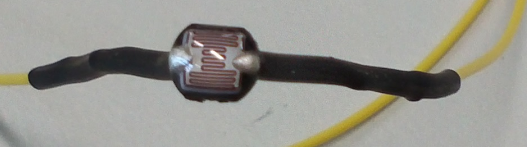
\includegraphics[width=0.9\columnwidth]{Abbildungen/Elektronik/LDR} 

}

{
\centering
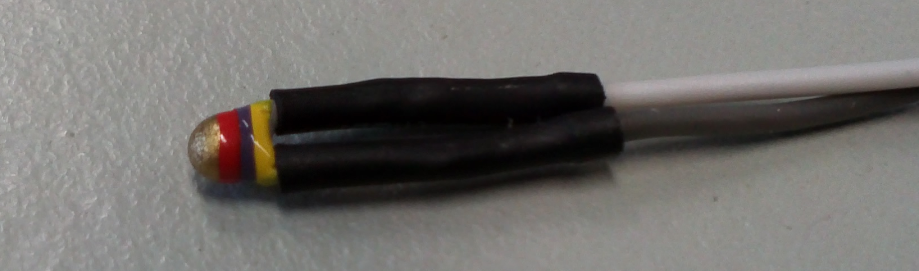
\includegraphics[width=0.9\columnwidth]{Abbildungen/Elektronik/NTC} 

}


\textbf{DCF 77}

Das DCF77-Modul empfängt das Mitteleuropäische Zeitsignal und verstärkt es. Um das Signal problemlos zu Empfangen wird hier ein interruptfähiger Eingang des Mikrocontrollers (1) verwendet. Durch regelmäßigen Empfang des DCF77 Zeitsignals ist die Genauigkeit des verbauten Quarz hinreichend genau.


\textbf{Spannungsversorgung}

Die Spannungsversorgung ist auf den Betrieb mit einem Gleichspannungsnetzteil (7~-~18$V$) ausgelegt und in die zwei Bereiche Elektronik und LED aufgeteilt. Der Bereich Elektronik wird von dem Spannungsregler auf dem Arduino Board versorgt. Die LEDs haben einen eigenen LM7805 Spannungsregler mit 1,5A Ausgangsstrom. An der Hohlsteckerbuchse am Rahmen kann alternativ ein Brückengleichrichter eingelötet werden, dieser verhindert die Verpolung des Netzteils und reduziert den Spannungsfall an den Spannungsreglern.
\end{multicols}

{
\centering 
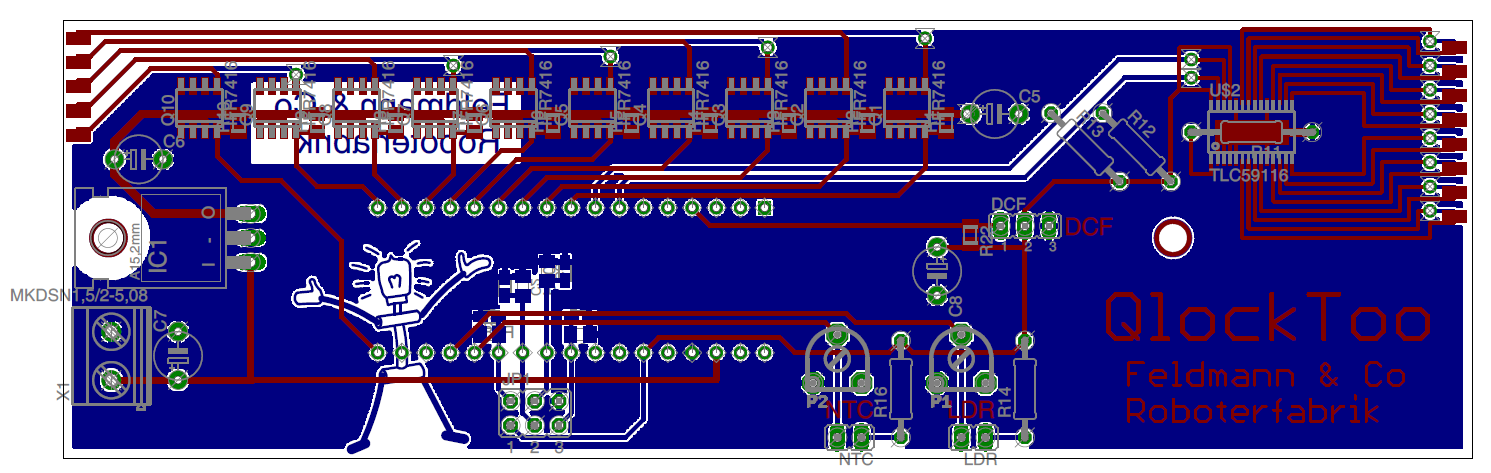
\includegraphics[width=\textwidth]{Abbildungen/Elektronik/Layout01} 
}
\begin{multicols}{2}

\textbf{Platinenlayout}

Das Platinenlayout wurde mit dem PCB Design Tool CADSoft Eagle erstellt. Die Leiterbahnen des Top-Layers sind in Rot dargestellt und die Leiterbahnen, sowie die Massefläche, des Bottom-Layer sind in Blau dargestellt. 
Der Arduino Micro wird mit zwei Buchsenleisten auf die Platine aufgesteckt und bildet mit seinem ISP-Stecker das höchste Bauteil. Die Stiftleisten für den 10 poligen und er 16-poligen Stecker zur LED-Matrix werden stirnseitig angelötet.

Die Platine wird aus einer zweiseitigen Fotoplatine erstellt. Hierzu werden Top- und Bottom-Film auf der Fotoplatine ausgerichtet und die Platine 3 Minuten mit UV-Licht belichtet. Im Entwicklerbad mit Natriumhydroxid wird der belichtete Fotolack abgewaschen.Die belichteten Stellen auf der Platine werden in einer Ätzanlage mit Eisentrichlorid entfernt. Je nach Güte des Ätzmittels verbleiben nach bereits 2 Minuten im Ätzbad nur noch die unter dem unbelichteten Fotolack liegenden Leiterbahnen. Im Nachgang wird die geätzte Platine nochmals vollständig belichtet, der Fotolack im Entwicklerbad abgewaschen und die Platine mit Kunststofflack beschichtet.


\end{multicols}

